\chapter{Konfigurationsmanagement}
\label{cha:konfigurationsmanagement}
Im Zusammenhang mit Docker und einem Softwareentwicklungsprozess werden oftmals zahlreiche weitere Werkzeuge genannt, die ähnliche Einsatzgebiete haben, oder in Kombination mit Docker den Prozess erheblich verbessern können.
In den folgenden Abschnitten werden die bekanntesten und am weitest verbreiteten Werkzeuge und deren jeweilige Einsatzzwecke vorgestellt.
Zusätzlich werden exemplarische Szenarien und die mögliche Kombination mit Docker aufgezeigt.

Die vorgestellten Werkzeuge dienen der Konfiguration der Entwicklungs- und Produktionsumgebung.
Wie~\autocite[29\psq]{Wolff201604} beschreibt, ließen sich diese Konfigurationen auch manuell vornehmen, doch damit treten erhebliche Probleme im Sinne der Testbarkeit, Reproduzierbarkeit und Automatisierung auf.
Ein noch größeres Problem stellt das implizite Wissen der Entwickler dar, das bei einer händischen Konfiguration nur verbal weitergegeben wird.
Selbst eine ausführliche Dokumentation löst dieses Problem nicht, da der Mensch im Gegensatz zum Computer dazu tendiert, fest definierte Abfolgen trotz genauer Spezifikation nicht fehlerlos durchzuführen, weshalb die Idee der Infrastrukturverwaltung in Versionsverwaltungssystemen entstanden ist.


\section{Infrastructure as Code}
\label{sec:infrastructureascode}
Da jede Anwendung eine Umgebung zur Ausführung benötigt und gerade in den letzten Jahren die Komplexität der Anwendungen im Hinblick auf die Anzahl und das Zusammenspiel zahlreicher Komponenten stark zugenommen hat, gibt es den Ansatz des \emph{Infrastructure as Code} \autocite{InfrastructureAsCode:online}.
Dabei werden, wie zuvor bereits beschrieben, die Vorteile von Versionsverwaltungssystemen auf die Infrastruktur einer Anwendung angewandt.
Die Anwendungsinfrasktruktur wird nicht mehr händisch aufgebaut, sondern in Quelltexten abgelegt, wodurch das tatsächliche Erstellen der Infrastruktur auf diverse Werkzeuge verteilt wird.

Dadurch können, wie in~\autocite[64\psqq]{Wolff201604} beschrieben, zahlreiche Vorteile erreicht werden:
\begin{itemize}
    \item Das System wird reproduzierbar, da manuelle Konfigurationsfehler vermieden werden.
    \item Bei einer konsequenten Durchführung entstehen idente Test- und Produktionsumgebungen, die sich bis zur Netzwerkebene nicht unterscheiden.
    \item Inkonsistent gewordene Systeme müssen nicht zwangsläufig repariert werden, wodurch sich Änderungen oder weitere Probleme ergeben können, sondern können entsorgt und sofort wieder aufgebaut werden.
    \item Die Infrastruktur ist nun reviewfähig, wodurch Probleme frühzeitig entdeckt werden. Unter reviewfähig ist hier zu verstehen, dass die Infrastruktur aufgrund der Darstellung in Quelltext von dritter Seite geprüft und validiert werden kann.
    \item Wenn zusätzlich zu Infrastructure as Code auch noch verstärkt mit Virtualisierungstechniken gearbeitet wird, lässt sich die Umgebung der Anwendung unter hoher Last aufgrund der replizierbaren Umgebung einfach skalieren. Dies bringt allerdings nur einen Vorteil, wenn die Anwendung auf eine horizontale Skalierung ausgelegt ist.
    \item Eine Dokumentation der gesamten Infrastruktur entsteht automatisch. Allerdings ohne dass sie aktualisiert werden muss, denn der Infrastruktur-Quelltext ist zugleich die Dokumentation.
    \item Durch diese Selbstdokumentation wird auch gewährleistet, dass an jede Softwareversion auch die dazu benötigte Infrastrukturversion gebunden wird. Diese Tatsache vereinfacht das Testen und das Ausrollen der Software um ein Vielfaches, da die Anforderungen an die Umgebung bekannt sind. Voraussetzung dafür ist allerdings, dass sich der Anwendungs- und Infrastrukturquelltext in einem gemeinsamen oder zumindest verknüften Repository der Versionsverwaltung befinden.
\end{itemize}
Damit dieses System funktioniert, dürfen Änderungen an der Infrastruktur allerdings \emph{nur} an den Konfigurationsdateien geändert werden. Da die Infrastruktur auf Basis dieser Konfiguration erstellt wird, gibt es keinen Datenrückfluss aus den Systemen in die Konfiguration.


\section{Werkzeuge}
\label{sec:konfigurationswerkzeuge}
Um die Verwaltung der Infrastruktur zu erleichtern, existieren zahlreiche Werkzeuge, von denen die wichtigsten im Folgenden beschrieben werden.

\subsection{Vagrant}
\label{sub:vagrant}
Die folgenden Informationen und Quelltext-Beispiele sind aus \autocite{Vagrant:online} entnommen.
Vagrant ist ein Verwaltungswerkzeug für virtuelle Maschinen (siehe~\cref{sec:vollvirtualisierung}).
Die Idee von Vagrant ist, bereits bestehende Virtualisierungslösungen wie VMware, VirtualBox oder AWS zu verwenden.
Diese werden mit Werkzeugen, die sich um die Bereitstellung von Software kümmern (vgl. \cref{sub:chef} oder \cref{sub:puppet}) zu fertigen virtuellen Maschinen für Entwickler oder Infrastrukturmanager erweitert.
Aufgrund dieses Aufbaus können virtuelle Maschinen sehr einfach erweitert und daher generisch verwendet werden.
Um nicht immer jede virtuelle Maschine komplett neu erstellen zu müssen, gibt es in Vagrant bereits vorgefertigte Schablonen für virtuelle Maschinen, sogenannte \emph{Boxen}, die als Basis verwendet werden können.

Vagrant verwendet dazu eine eigene auf Ruby basierende \emph{Domain Specific Language} (DSL), die in den so genannten \emph{Vagrantfiles} Einsatz findet.
Das Vagrantfile wird mit dem Quelltext mitversioniert und bietet den Entwicklern reproduzierbare, portable und plattformunabhängige Entwicklungsgeräte.
Das Konzept der Vagrantfiles ist auch in Docker (siehe~\cref{sec:dockerfiles}) wiederzufinden.
Dadurch verliert der bekannte Satz ``But it works on my machine!'' stark an Bedeutung und Relevanz.
Anwendungen, die in der von Vagrant zur Vefügung gestellten Umgebung laufen, laufen immer auch in einer identen Umgebung, die sehr einfach mit Vagrant zur Verfügung gestellt werden kann.

\subsubsection{Beispiel eines Apache-Webservers mit Vagrant}
Mit den folgenden Skripten wird ein Apache-Webserver in einer virtuellen Maschine gestartet.
\cref{lst:vagrant-bootstrap} ist ein ausführbares Shell-Skript, welches den Apache-Webserver installiert und vom Vagrantfile verwendet wird.
\lstinputlisting[caption=Skript zum Installieren des Apache-Webservers (\emph{bootstrap.sh}),label={lst:vagrant-bootstrap}, language=bash]{listings/bootstrap.sh}
Der Vagrantfile in \cref{lst:vagrantfile} beschreibt, dass die Box mit dem Namen \emph{hashicorp/precise64} verwendet wird und zum Erstellen der fertigen virtuellen Maschine ein Shell-Skript namens \emph{bootstrap.sh} ausgeführt werden soll.
Der Parameter \lstinline{"`2"'} in der ersten Zeile gibt die Version des Vagrant-Konfigurationsobjekts an.
Dadurch kann Vagrant die Rückwärtskompatibilität zu älteren Parametern gewährleisten.
\lstinputlisting[caption=Vagrantfile,label={lst:vagrantfile}, language=Ruby]{listings/Vagrantfile}

Der Haupteinsatzzweck von Vagrant liegt im Verwalten von virtuellen Maschinen für Entwickler, die die Produktionsumgebung spiegeln und ein plattformunabhängiges Entwickeln ermöglichen.
Ein besonders nützlicher Anwendungsfall für Vagrant-Boxen sind Legacy-Systeme, für die eine vorkonfigurierte Entwicklungsumgebung benötigt wird, die auf keinem aktuellen Entwicklerrechner mehr verwendet wird.
So kann für einfache Bug-Fixes eine Vagrant-Entwicklerbox gestartet werden, ohne dass am Entwicklerrechner nicht mehr benötigte Werkzeuge installiert sein/werden müssen.


\subsection{Chef}
\label{sub:chef}
Wie auf der offiziellen Homepage \autocite{Chef:online} von Chef~Software,~Inc.\ beschrieben, ist Chef ein Werkzeug zur Infrastrukturautomatisierung.

\autocite{Wolff201604} liefert eine sehr gute und prägnante Einführung in das Werkzeug Chef.
Im Gegensatz zu einer Sammlung von Shell-Skripten, bietet Chef ein Framework für die Konfiguration und das Erstellen von Systemen.
Bestehende Funktionalität wird von Chef angeboten und die Konfigurationen werden in einer Meta-Sprache geschrieben.
Dies hat den Vorteil, dass Sonderfälle minimiert werden, da sie von Chef übernommen werden. Zum Beispiel muss ein schon vorhandenes veraltetes System nicht komplett entfernt und neuinstalliert werden, sondern kann durch das Aktualisieren der Anforderungen auf den neuen, aktuellen Zustand gebracht werden.

Chef verwendet ebenso wie Vagrant eine Ruby-DSL, die in den so genannten \emph{Rezepten} (\emph{Recipes}) Verwendung findet.
Diese Rezepte definieren die Anforderungen an die einzelnen Teile der Infrastruktur. Darin werden Konfigurationsdateien, Benutzer, Anwendungen, Plug-ins und weitere Abhängigkeiten spezifiziert.
Da diese Rezepte mit steigender Komplexität des Systems an Übersichtlichkeit verlieren, gibt es die Gruppierung dieser in \emph{Kochbücher} (\emph{Cookbooks}).
Diese Kochbücher fassen mehrere Rezepte zusammen und bieten die Möglichkeit der \emph{Vorlagen} (\emph{Templates}) für Konfigurationsdateien, wodurch zahlreiche Server unterschiedlich parametrisiert werden können.
Chef kann entweder in einem "`Solo"'-Operationsmodus betrieben werden oder als "`Chef Zero"' für Testzwecke. Zusätzlich gibt es auch die Option einer Client-Server-Umgebung, in der ein Chef-Server das Management der Konfigurationen übernimmt.
Von dort aus können mit geringem Aufwand neue Teile der Infrastruktur gestartet und bestehende gewartet werden. Dazu existieren als Erweiterung zu Chef Werkzeuge wie Knife\footnote{\url{https://docs.chef.io/knife.html}}.

\subsection{Puppet}
\label{sub:puppet}
Der Zweck von Puppet ist wie bei Chef die Automatisierung der IT-Infrastruktur. \autocite{Wolff201604} liefert einen Vergleich der beiden Werkzeuge.

Puppet verfolgt ebenso den Ansatz einer Beschreibung des Endzustandes des Systems, anstelle von Installationsskripten.
Im Gegensatz zu Chef werden bei Puppet die Konfigurationen rein deklarativ beschrieben.
Daher reicht als Beschreibungsformat \emph{JSON}.
Die möglichen Anweisungen können mit Ruby-Code erweitert werden.
Dadurch wird wie bei Chef eine sehr hohe Flexibilität erreicht, viele der Aufgaben sind allerdings durch die deklarative Beschreibung leichter verständlich.
Diese Unterschiede in der Syntax reflektieren die ursprüngliche Anwendergruppe.
Chef war durch die starke Verwendung von Ruby eher für Entwickler gedacht.
Puppet hingegen durch die deklarative Beschreibung der Konfigurationen für Systemadministratoren, die an Konfigurationsdateien und die Kommandozeile gewöhnt sind.

In \autocite{chef-vs-puppet:online} wird beschrieben, dass der Chef-Ansatz eine höhere Flexibilität ermöglicht, dies allerdings mit einer steileren Lernkurve einhergeht.
Der modellgetriebene Ansatz von Puppet ist zwar simpel, liefert jedoch im Gegensatz zu einer prozeduralen Systembeschreibung Interpretationsspielraum.
Beim Erstellen des Systems muss sichergestellt werden, dass die Kommandos jedes Mal gleich erzeugt werden, was durch Änderungen am Algorithmus nicht garantiert werden kann.

\autocite{chef-vs-puppet-revisited:online} liefert eine Einführung in die weiterführenden Systeme und Werkzeuge der Firmen Chef\footnote{\url{https://www.chef.io/about/}} und Puppet\footnote{\url{https://puppet.com/company}}.

\subsection{SaltStack}
\label{sub:saltstack}
SaltStack ist eine Open-Source-Softwarelösung für die Konfiguration und Automatisierung von Servern.
Die folgenden Informationen stammen aus \autocite{SaltStack:online}.

SaltStack basiert auf einer Master-Slave-Architektur, bei der sich die Slaves (in SaltStack \emph{Minions} genannt) beim Master registrieren und ab diesem Zeitpunkt steuern lassen.
Der einfachste Anwendungsfall ist die Ausführung von Kommandos auf zahlreichen verteilten Servern.
Dazu sendet der Master die Kommandos an die Minions, die diese ausführen.
Um Reproduzierbarkeit und dadurch Konfigurationsmanagement zu erreichen, werden die Konfigurationen mit YAML in SLS-Dateien (SaLt State) definiert und an die Minions verteilt.
Diese States werden für einzelne Gruppen definiert, wobei jeder Minion seine Gruppenzugehörigkeit weiß und die zu ihm passenden States anwendet.

Laut \autocite{SaltStack-Event:online} bietet SaltStack die Möglichkeit von ereignisgetriebenen Infrastrukturen.
Alle Aktionen im SaltStack-System führen zu Ereignissen, auf die reagiert werden kann.
So entstehen reaktive Infrastrukturen, die sich selbst bereitstellen, verwalten und reparieren können.
Dazu lassen sich für Ereignisse und Ereignisgruppen Beobachter und Reaktoren definieren, die wissen, welche Aktionen bei welchen Ereignissen oder Ausnahmen zu tätigen sind.
So kann zum Beispiel bei einer zu voll werdenden Festplatte neuer Speicher zur Verfügung gestellt, oder der bereits vorhandene Speicher defragmentiert werden.
Weiters sind auch Szenarien möglich, bei denen bei steigender Last oder Knotenausfall neue Server bereitgestellt werden.

\subsection{Ansible}
\label{sub:ansible}
Wie die zuvor beschriebenen Werkzeuge bietet auch Ansible die Automatisierung von IT-Systemen.
Die folgenden Informationen stammen aus \autocite{Ansible:online}.

Die Konfigurationsdateien in Ansible werden Playbooks genannt und sind wie bei SaltStack in YAML geschrieben.
Der große Unterschied bei Ansible ist, dass kein Ansible-Service auf den Client laufen muss, da Ansible die Kommandos über SSH, WinRM oder Cloud-APIs ausführt.
Lediglich auf dem Master ist Ansible installiert.
Dieser weiß zusätzlich über ein in Ansible \emph{Inventory} genanntes Verzeichnis Bescheid, welche Clients im System verfügbar sind und wie er diese anzusteuern hat.

Die eben beschriebene CLI-Funktionalität wird durch Ansible Tower um ein grafisches Benutzerinterface erweitert.
Dadurch können die Ansible-Aufgaben sehr einfach verwaltet und dem gesamten Team zur Verfügung gestellt werden.

Mit der Entwicklung von Ansible wurde erst 2012 gestartet, wodurch viele der Probleme aus anderen Systemen behoben und verbessert wurden \autocite{Wolff201604}. Dieser technisch besseren Basis steht allerdings der Nachteil der kleineren Benutzergruppe gegenüber.

\subsection{Packer}
\label{sub:packer}
Packer ist ein Werkzeug zum Erstellen von vorkonfigurierten virtuellen Maschinen.
In \autocite{Packer:online} werden Anwendungsszenarien und Einsatzmöglichkeiten gezeigt.

Das quelloffene Kommandozeilenwerkzeug verwendet Konfigurationsmanagementwerkzeuge wie Chef oder Puppet zum Konfigurieren und Erstellen von virtuellen Maschinen.
Der große Vorteil darin besteht in der Abstraktion des Zielsystems.
Packer erstellt virtuelle Maschinen auf Basis von Konfigurationsdateien, wobei die Zielplattform unabhängig von der Konfiguration ist.
Dadurch kann eine beinahe idente virtuelle Maschine für die Produktion, sowie für die Entwickler zur Verfügung gestellt werden, indem auf Basis einer Konfiguration beispielsweise virtuelle Maschinen für Amazon AWS (Produktion) und Vagrant (Entwicklung) erstellt werden.

Packer abstrahiert die Plattformunterschiede, wodurch bei der Konfiguration von virtuellen Maschinen die Zielplattform nicht feststehen muss.
Diese lässt sich bei der Verwendung von Packer im Nachhinein sehr einfach anpassen.

Durch die Verwendung von Packer wird eine zusätzliche Abstraktionsstufe geschaffen, die Vendor-Lock-Ins reduziert.
Auch Docker-Container können mithilfe von Packer erzeugt werden.
Diese Möglichkeit erzeugt dasselbe Resultat wie die Verwendung von Dockerfiles (siehe \cref{sec:dockerfiles}), wobei keine Bindung an Docker entsteht, allerdings ein zusätzliches Werkzeug verwendet wird, das nicht in das Docker-Ökosystem integriert ist.


\section{Kombinationsmöglichkeiten der Werkzeuge}
\label{sec:werkzeugkombinationsmoeglichkeiten}
Eine sehr durchdachte Kombination der eben vorgestellten Werkzeuge befindet sich bei der Firma npm Inc.\footnote{\url{https://www.npmjs.com/about}} im Einsatz.
npm ist der Paketmanager für die serverseitige JavaScript-Runtime Node.js.
Zusätzlich existieren die freie npm-Registry und Kommandozeilenwerkzeuge zum Verwalten der JavaScript-Pakete.
Die Firma npm Inc.\ entwickelt diese und hostet die Registry.
Der starke Open-Source-Ansatz von npm führte zu \autocite{npm-deployment:online}, worin beschrieben wird, welche Werkzeuge beim npm-Deployment im Einsatz sind. Daraus entstammen die folgenden Überlegungen.

\lstinputlisting[caption=Deployment-Prozess bei npm,label={lst:npm-deploy},language=bash]{listings/npm-deploy.sh}
Die Motivation des Deployment-Prozesses von npm liegt in der höchstmöglichen Simplizität für die Entwickler.
Daraus resultiert ein häufigeres Deployment, da nicht darüber nachgedacht werden muss, ob ein Deployment momentan überhaupt möglich ist.
In \cref{lst:npm-deploy} ist der gesamte Deployment-Aufwand dargestellt.
Ein git-Push auf den production-Branch genügt um den neuen Code samt Infrastruktur zu veröffentlichen.

In \cref{fig:configurationtools-npm} ist dargestellt, welche Aufgaben die Werkzeuge des Konfigurationsmanagements dabei übernehmen.
Die gesamte npm-Infrastruktur läuft auf ca.\ 120 virtuellen Maschinen in der Amazon-Cloud.
Um den Deployment-Prozess zu beschleunigen, wird von Packer in \circled{0} ein Basis-VM-Image mit Ubuntu erstellt.
Darin befindet sich bereits eine LTS-Version von Node.js als Laufzeitumgebung und das npm-interne Monitoring-System.

\emph{Terraform\footnote{\url{https://www.terraform.io/}}} kommt als nächstes Werkzeug, zum Einsatz.
Terraform ist ein weiteres Werkzeug zur Verwaltung von Infrastruktur als Code.
Der Haupteinsatzzweck liegt in der deklarativen Verwaltung von Cloud-Ressourcen.
Terraform dient dabei als Abstraktionsschicht zu den Cloud-Providern.
Bei npm wird nun das von Packer erstellte Basis-Image von Terraform verwendet \circled{1}, um eine virtuelle Maschine in der Amazon-Cloud zu erstellen \circled{2}.

Danach wird Ansible mit einem Playbook aufgerufen, das die benötigten Services installiert und startet, Webhooks konfiguriert und zum Start der npm-Services die Deployment-Skripte ausführt \circled{4}.
npm verwendet dazu keine externen Werkzeuge, sondern Bash-Skripte, die auch händisch gestartet werden können.
Zur Konfiguration wird als (etcd\footnote{\url{https://github.com/coreos/etcd}}) als Datenbank verwendet.
Ein weiterer Grund gegen ein Werkzeug ist im Fall von npm die Einbindung in den internen Slack-Bot, über den der gesamte Deployment-Prozess beobachtet und angestoßen werden kann.

\begin{figure}[htbp]
    \centering
    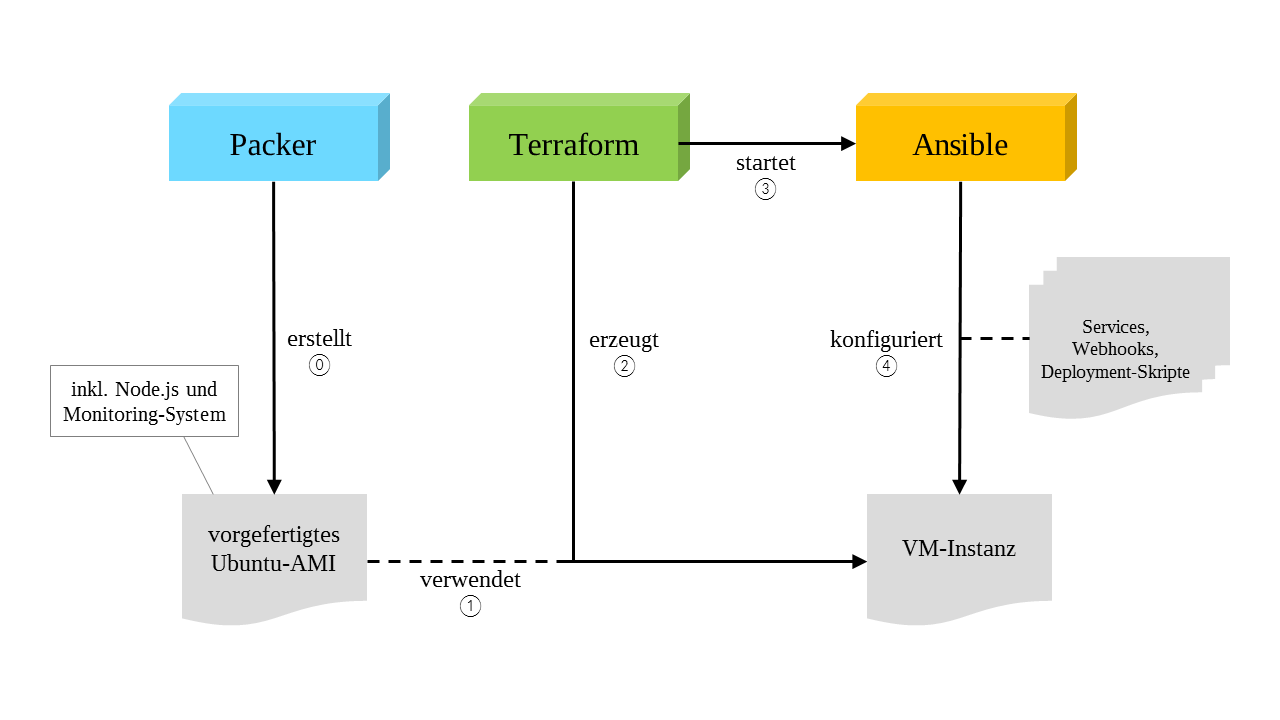
\includegraphics[width=0.9\linewidth,clip]{images/npm-deployment}
    \caption{Packer, Terraform und Ansible im Einsatz bei npm}
\label{fig:configurationtools-npm}
\end{figure}

%Nach dem Start und der Konfiguration der virtuellen Maschine wird diese zuerst in einen Canary-Modus im Load-Balancer geschaltet.
%Dieser testet unter sehr geringer Produktivlast die Funktionsfähigkeit des Systems, bevor der neue Knoten tatsächlich unter volle Produktionslast geschaltet wird.
